\chapter{Results}
\label{chap:results}

When an algorithm is being designed, its evaluation against existing solutions belongs to important stages of its development. This chapter describes this stage, informing about a data set used to debug and improve our solution, and the method of comparison with other solutions, such as fermi-kit and GATK. The last part of the chapter covers certain variants that proved to be interesting when examined by our algorithm.

\section{Test Data Set}
\label{sec:test-data-set}

The algorithm was tested on the first 40 megabases of chromosome 1 of the human genome. The test set is a high-coverage one and was obtained from the 1000 Genome Project. Except the input reads \cite{testreads}, variants called by fermi.kit and GATK are also available in form of VCF files \cite{testvcf}. The VCF files were used as a measure of algorithm quality. Since our algorithm also requires a reference sequence to work, we took the GRCh37 version \cite{testref}.

The input read set consists of 12475011 reads with lengh of 151 bases. Figure \ref{fig:test-kmer-frequency-distribution} shows k-mer frequency distribution of the set with k-mer size of 21 bases. The shape of the graph, when compared to Figure \ref{fig:kmer-frequency-distribution} suggests that the set contains read errors. Hence, an error correction step was applied.

% \begin{figure}[h]
%	\centering
%	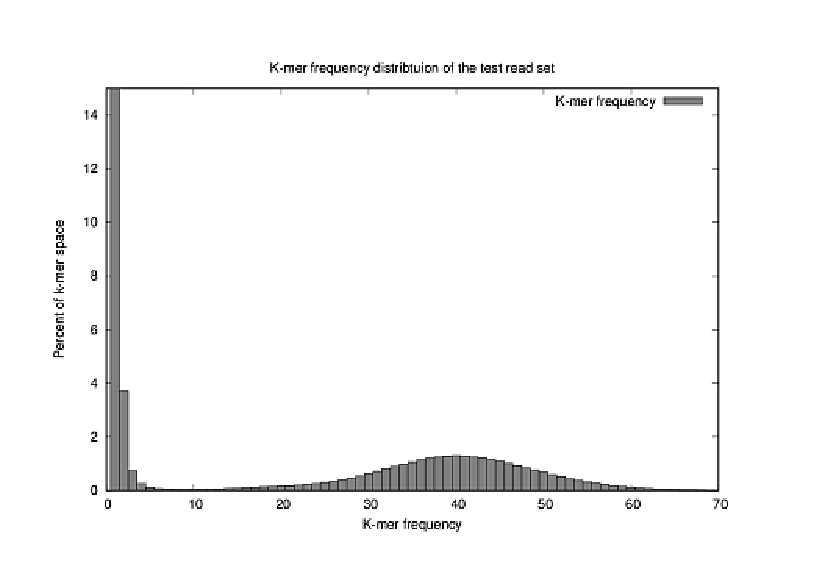
\includegraphics{img/test-kmer-frequency-distribution.pdf}
%	\caption{K-mer frequency distrubtion of the raw input read set}
%	\label{fig:test-kmer-frequency-distribution}
% \end{figure}


As Table \ref{tab:test-correction} indicates, the error correction process removed and shortened certain amount of reads. About 21 \% of the input reads was subject to repairs. Figure \ref{fig:test-repair-frequency} shows a distribution of the number of repaired bases per read, not including effects of read shortage. It is clear, that about 21 \% of all reads received a base correction, and that, in most cases, only several bases were fixed. 

\begin{table}[h]
\begin{center}
\caption{Statistics related to error correction of the test data set}
\label{tab:test-correction}
\begin{tabular}{| c | c | p{5cm} |}
\hline
Category & Value & Percentage \\
\hline
Total reads & 12475011 & - \\
\hline
Removed & 64653 &  $0.52$ \% of all reads. \\
\hline
Shortened & 944 & $0.0076$ \% of all reads \\
\hline
Total bases & 1880123991 & - \\
\hline
Bases repaired & 5098764 &  $0.27$ of all bases \\
\hline
\end{tabular}
\end{center}
\end{table}

\begin{figure}[h]
	\centering
	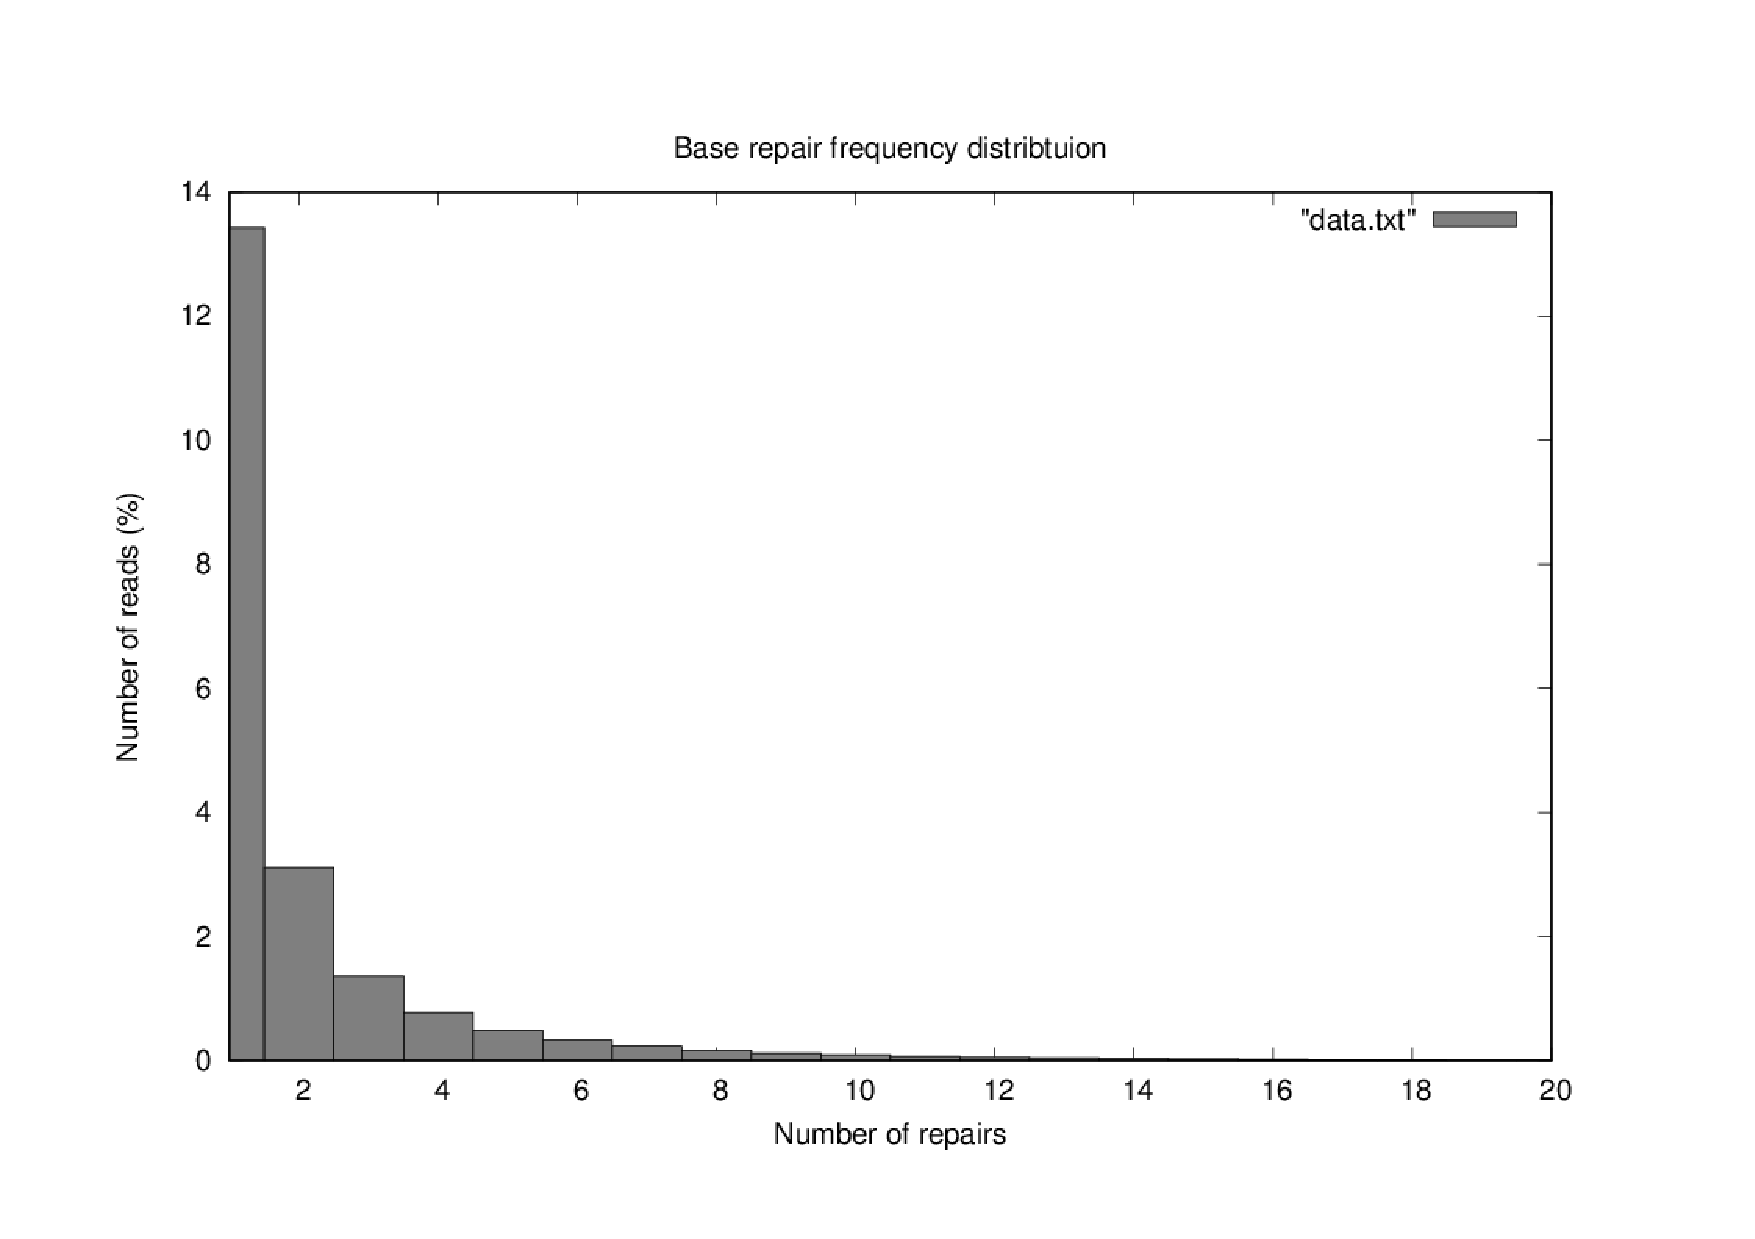
\includegraphics{img/test-repair-frequency.pdf}
	\caption{Distribution of a number of repaired bases in a single read}
	\label{fig:test-repair-frequency}
\end{figure}

Figure \ref{fig:test-kmer-frequency-distribution2} shows the k-mer frequency distribution of the corrected read set. Although quite far from perfect, the graph shape definitely resembles the ideal one better then in case of the raw  read set. 

% \begin{figure}[h]
%	\centering
%	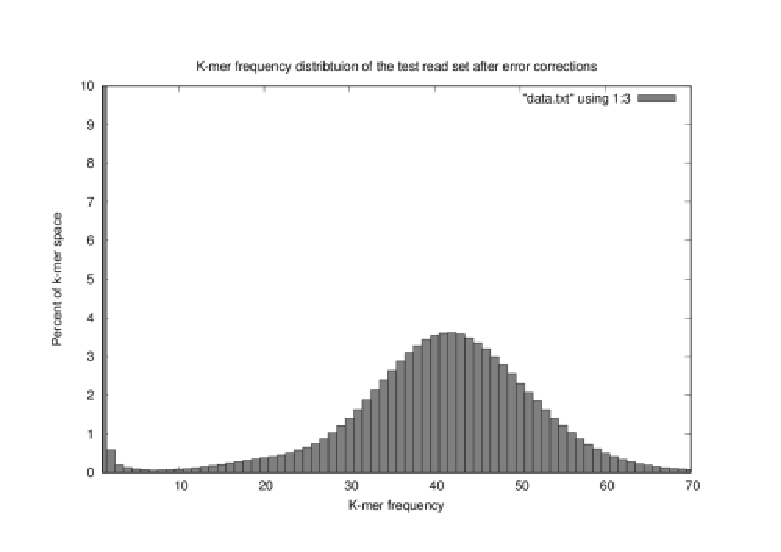
\includegraphics{img/test-kmer-frequency-distribution2.pdf}
%	\caption{K-mer frequency distrubtion of the corrected read set}
%	\label{fig:test-kmer-frequency-distribution2}
% \end{figure}

As described in Section \ref{sec:data-preprocessing}, not all input reads, even from the corrected set, can be processed by our algorithm. Table \ref{tab:corrected-set-categories} summarizes numbers of reads unacceptable for various reasons. The preprocessing phase removed nearly one fifth of the corrected data set (18.99 \%). Most of the reads were removed due to being possible duplicates (87.65 \%). Quite a large portion of  reads were not accepted because of their low mapping quality (12.97 \%). Also, about 3 \% of all the reads were shortened in order to remove soft-clipped regions.

\begin{table}[h]
\begin{center}
\caption{Categories of reads present within the corrected test data set}
\label{tab:corrected-set-categories}
\begin{tabular}{| c | c | p{5cm} |}
\hline
Name & Value & Percentage \\
\hline
Total reads & 12410475 & - \\
\hline
Bad reads & 2357002  & $18.99$ \% of all reads \\
\hline
Low MAPQ & 305588 & $12.97$ \% of bad reads \\
\hline
Unmapped & 5020 & $0.21$ \% of bad reads \\
\hline
Supplementary & 33621 & $1.43$ \% of bad reads \\
\hline
Duplicate & 2065795 & $87.65$ \% of bad reads \\
\hline
Soft-clipped & 305209 & $3.04$ \% of accempted reads \\
\hline
\end{tabular}
\end{center}
\end{table}

\section{Quality Evaluation}
\label{sec:quality-evaulation}

In order to evaluate quality of the algorithm, VCF files generated by it were compared to those generated by the following variant calling toolchains:
\begin{itemize}
\item \textbf{GATK}. These VCFs were taken as referepnce points, since the method used by GATK should be very similar to our algorithm. Hence, results of all algorithms were compared against them. Necessary VCF files are part of the test data set.
\item \textbf{Fermi.kit}. Unlike GATK and our algorithm, fermi.kit's assembly algorithm is based on the OLC concept. VCFs generated for the test region are part of the test data set.
\item \textbf{Fermi.kit on regions}. This is a combination of the OLC approach used by Fermi.kit and the short region one adopted by our algorithm (and also by GATK). The fermi.kit assembly algorithm was run on exactly the same regions as our algorithm. The aim of this test case was to force the Fermi.kit to minimize differences of outputs generated by DBG and OLC algorithms.
\item \textbf{samtools mpileup, bcftools call}. A quite simple variant caller implemented by SAMtools and BCFtools commands \cite{samtools}.
\end{itemize}

Results generated by these algorithms were compared to those of GATK using a tool named rtgeval. Rtleval is a wrapper for RTG's vcfeval, a sophisticated open source variant comparison tool developed by Realtime Genomics. It simplifies the use of vcfeval and potentially helps to get consistent results given VCFs produced by different variant callers \cite{rtgeval}.

Rtgeval uses quite simple terminology. Basicaly, it accepts two VCF files: test set and truth set. The truth set is a VCF file generated by an assembly algorithm we trust (GATK in our case). The test set VCF is produced by the algorithm to be tested. The evaluation is done separately for SNPs and indels and each variant is sorted into one of three categories:
\begin{itemize}
\item \textbf{True positive (TP)}. The variant is present in both sets.
\item \textbf{False negative (FN)}. It is present in the truth set only.
\item \textbf{False positive (FP)}. It can be found only in the test set.
\end{itemize}

Rtgeval can compare VCF files in three different modes: positional, allelic and genotypic. The positional mode is quite intuitive; the tool is determining whether the same varaints are present at approximately the same position inside both test and truth set. If the positions difference does not exceed 10 bases, the variants are considered true positives. Otherwise, either false negative, or fale positive is reported. In allelic mode, the tool focuses on biallelic variants and evaluates whether they are correctly detected by both tested algorithms. The genotyping mode compares genotype and phasing information of the variants.

\subsection{Positional}
\label{subsec:positional-results}

\begin{table}[h]
\begin{center}
\caption{Positional comparison of results generated by our algorithm}
\label{tab:positional-results}
\begin{tabular}{| c | c | c | c | p{3cm} |}
\hline
/ & Fermi.kit & Fermi.kit (regions) & mpileup & Our algo \\
\hline
SNP TP & 45241 (89,3 \%) & 47650 (94 \%) & 49201 (97.1 \%) & 48117 (94.96 \%) \\
\hline
SNP FN & 5432 (10,7 \%) & 3043 (6 \%) & 1472 (2.9 \%) & 2556 (5.04 \%) \\
\hline
SNP FP & 385 (0,76 \%) & 1441 (2,84 \%) & 2090 (4.12 \%) & 803 (1.58 \%) \\
\hline
INDEL TP & 7853 (71, 6 \%) & 9802 (89,4 \%) & 8707 (79.39 \%) & 9468 (86.43 \%) \\
\hline
INDEL FN & 3114 (28,4 \%) & 1365 (10,6) \%) & 2260 (20.61 \%) & 1499 (13.57 \%) \\
\hline
INDEL FP & 250 (2,28 \%) & 835 (7,61 \%) & 1412 (12.95 \%) & 1242 (11.32 \%) \\
\hline
\end{tabular}
\end{center}
\end{table}

\begin{itemize}
\item describe algorithms and software to evaluate the results (fermikit, fermikit run at individual regions, GATK, mpileup of samtools, rtgeval for evaluation),
\item Show the position-based and genotype results of rtgeval.
\item describe interesting variants (variants that are not found by other software, explain some false negatives, demonstrate that graph optimizations actually revealed some variants...).
\end{itemize}
